\subsubsection{Some Important Linear Filters}
\label{subsubsection:kernels}

The following section outlines the characteristics of some linear filters that are used commonly in image processing and thus are important to be aware of. 

\textbf{A Box Filter}, also known as a moving average filter, is a linear filter whose kernel has uniform weights. The output of this filter is just the average of the neighborhood of pixels that it covers. Figure \ref{fig:box_kernel} shows an example box filter kernel whose size is 3, by passing this filter over an image its sharpness is reduced because average values that the filter outputs flattens out difference in image intensity. In Figure \ref{fig:pug_blur} this reduction in sharpness, or blurring though subtle, can be observed. A box filter is also a simple method of removing noise in an image because is diminished the effect of intensity spikes in an image. 

\begin{figure}[H]
   \centering
   \[k =
     \frac{1}{9}
   \begin{bmatrix}
      1 & 1 & 1 \\
      1 & 1 & 1 \\
      1 & 1 & 1
   \end{bmatrix}
   \]
   \caption{3x3 Box Filter Kernel}
   \label{fig:box_kernel}
\end{figure}

% DOG BOX FILTERED%
\begin{figure}[H]
    \centering
    \begin{subfigure}[b]{0.3\textwidth}
        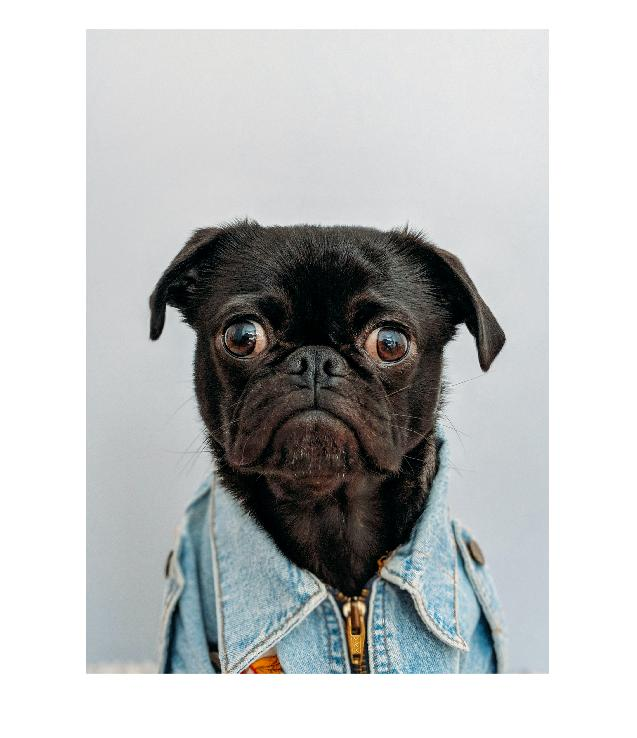
\includegraphics[width=\textwidth]{pug_resized}
        \caption{Img: Charles Deluvio}
        \label{fig:pug_noise}
    \end{subfigure}
    \begin{subfigure}[b]{0.3\textwidth}
        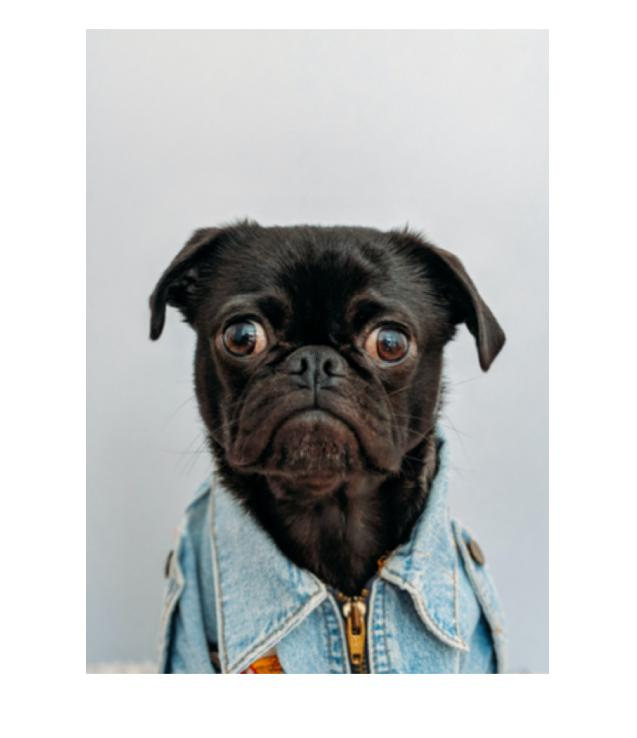
\includegraphics[width=\textwidth]{pug_blur}
        \caption{Blurred pug}
        \label{fig:pug_denoised}
    \end{subfigure}
    \caption{Application of a 17x17 Box filter to blur image.}
    \label{fig:pug_blur}
\end{figure}

\textbf{The Gaussian Kernel} is a significant kernel in image processing as it is good at filtering out noise. This kernel models the Gaussian function (see Section \ref{section:gaussian}) or normal distribution. It works in a similar fashion to the moving average filter but is superior at filtering noise as it addresses two properties about images that are generally true \cite{udacity_cv}, 

\begin{enumerate}
    \item The 'real' value, the value that the pixel should be were it not for noise, is probably the same or similar to its neighbours. 
    \item Each pixel of noise in an image is added independently.
\end{enumerate}

The Gaussian addresses both of these qualities by having high value coefficients at the filter's centre and lower values tapering out to the edges of the filter (Figure \ref{fig:gauss_kernel}) meaning that values spatially closer together are more strongly correlated than those further away from the reference pixel. Figure \ref{fig:pug_noise} shows how a Gaussian kernel effectively removes Gaussian noise (section \ref{section:gaussian}) an image. Figure \ref{fig:gauss_kernel} shows an example of a Gaussian kernel and how the filter coefficients decrease from the centre outwards.

% SOBEL FILTER APPLICATION
\begin{figure}[H]
    \centering
    \begin{subfigure}[b]{0.3\textwidth}
        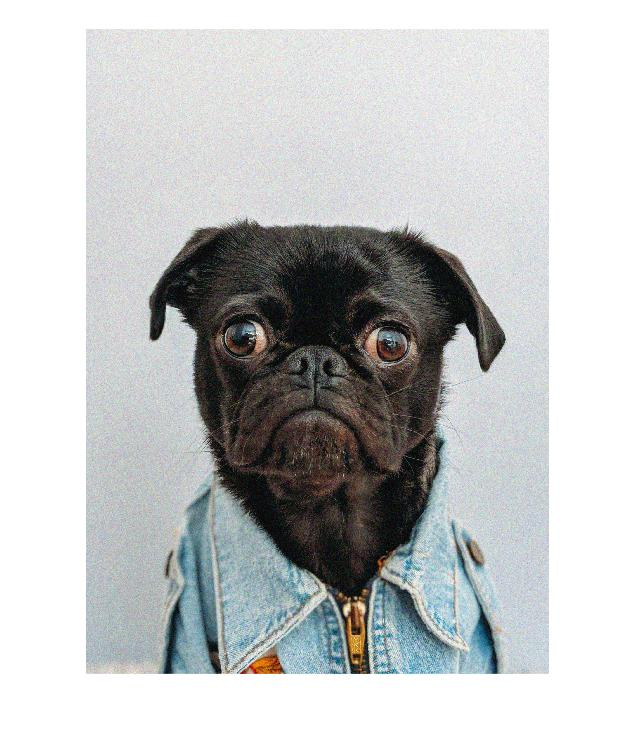
\includegraphics[width=\textwidth]{pug_noise}
        \caption{Noisy pug}
        \label{fig:pug_noise}
    \end{subfigure}
    \begin{subfigure}[b]{0.3\textwidth}
        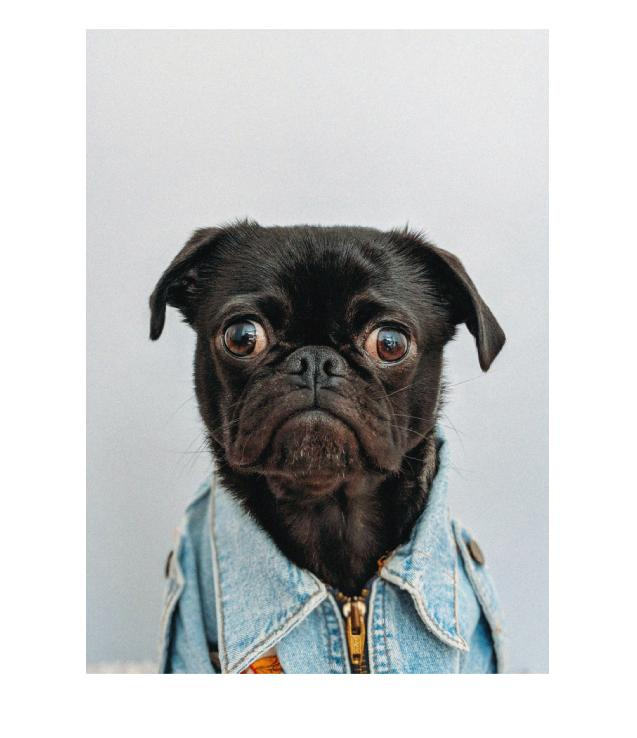
\includegraphics[width=\textwidth]{pug_denoised}
        \caption{Denoised pug}
        \label{fig:pug_denoised}
    \end{subfigure}
    \caption{Application of a 7x7 Gaussian filter to denoise image.}
    \label{fig:pug_noise}
\end{figure}


\begin{figure}[H]
    \centering
    \[k =
    \begin{bmatrix}
       0 & 0 & 0 & 0 & 0 & 0 & 0 \\
       0 & 0 & 0 & 0.0002 & 0 & 0 & 0 \\
       0 & 0 & 0.0113  & 0.0837 & 0.0113  & 0 & 0 \\
       0 & 0.0002 & 0.0837 & 0.6187 & 0.0837 & 0.0002 & 0 \\
       0 & 0 & 0.0113 & 0.0837 & 0.0113 & 0 & 0 \\
       0 & 0 & 0 & 0.0002 & 0 & 0 & 0 \\
       0 & 0 & 0 & 0 & 0 & 0 & 0 \\
    \end{bmatrix}
    \]
    \caption{7x7 Gaussian Filter Kernel, Sigma = 0.5}
    \label{fig:gauss_kernel}
\end{figure}

\textbf{Sobel Operators}, or Sobel-Feldman operators, are used to isolate edges in digital images by approximating the gradient function of the image in both the x and y direction with respect to pixel intensity \cite{sobel}. They are most commonly used on grayscale images. It's useful to be able to isolate edges in an image as it helps to identify distinct objects in an image. The filters approximate the gradient of an image because where an image has constant values the output of the kernel is 0 and where an edge is encountered the output will be a large positive or negative value, the structure of the Sobel kernels is shown in Figure \ref{fig:sobel_filters}.

In Figure \ref{fig:sobel_apply2} the gradients in the x and y directions are shown and the the final frame shows the image's gradient magnitude. The gradient magnitude is a scalar value representing size of rate of change in intensity of the image, it is the length of the vector between the derivate vectors in the x and y directions and is calculated 

\begin{equation}
|\triangledown f(x,y)| = \sqrt{\bigg (\frac{\delta f(x,y)}{\delta x} \bigg )^2 + \bigg (\frac{\delta f(x,y)}{\delta y} \bigg )^2}
\end{equation}

where $f(x,y)$ the image being filtered. This final result shows the edges in the image that the Sobel filters were able to isolate.

% SOBEL MASKS
\begin{figure}[H]
    \begin{subfigure}[b]{0.49\textwidth}
      \[k_x =
      \begin{bmatrix*}[l]
       -1 & 0 & 1 \\
        -2 & 0 & 2 \\
        -1 & 0 & 1
      \end{bmatrix*}
      \]
      \caption{Horizontal Sobel filter}
  \end{subfigure}
  \begin{subfigure}[b]{0.49\textwidth}
    \[ k_y = 
      \begin{bmatrix}
        -1 & -2 & -1 \\
        0 & 0 & 0 \\
        1 & 2 & 1
      \end{bmatrix}
      \]
      \caption{Vertical Sobel filter}  
  \end{subfigure}
      \caption{Sobel Filters}
      \label{fig:sobel_filters}
  \end{figure}

  \begin{figure}[H]
    \centering
    \begin{subfigure}[b]{0.45\textwidth}
        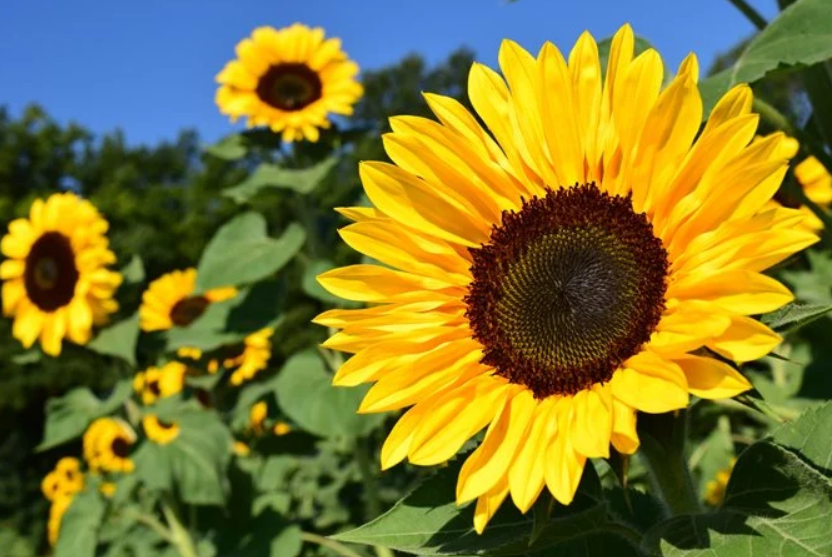
\includegraphics[width=\textwidth]{litreview/imageprocessing/linearfiltering/kernels/sunflowers}
        \caption{Img: Garden Design}
    \end{subfigure}
    \begin{subfigure}[b]{0.45\textwidth}
        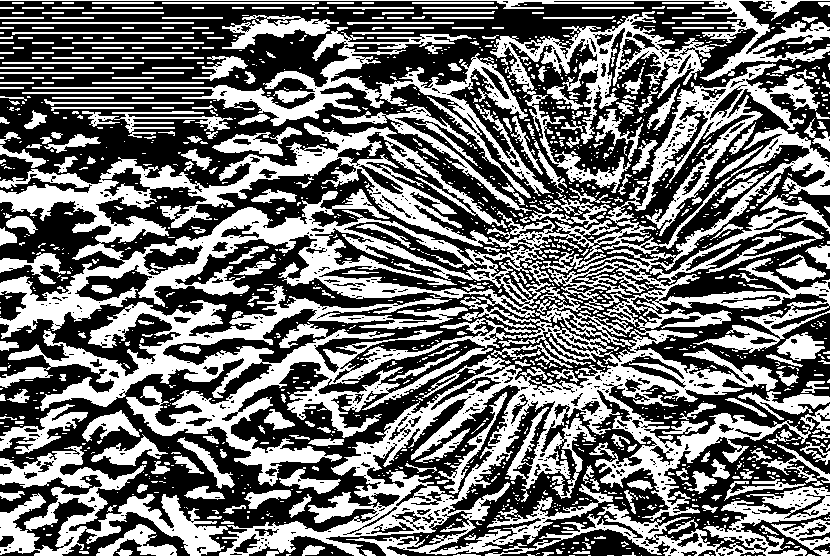
\includegraphics[width=\textwidth]{litreview/imageprocessing/linearfiltering/kernels/sunflowers_x}
        \caption{Vertical rate of change}
        \label{fig:vert}
    \end{subfigure}
    \begin{subfigure}[b]{0.45\textwidth}
        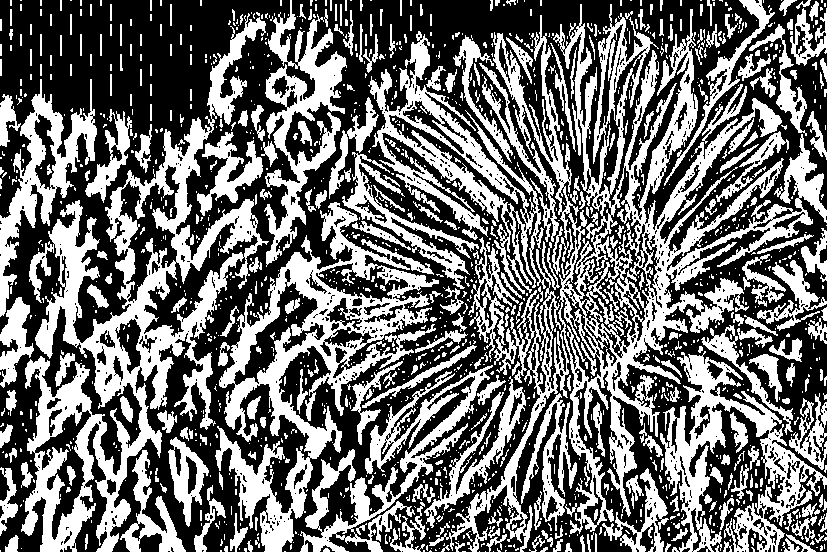
\includegraphics[width=\textwidth]{litreview/imageprocessing/linearfiltering/kernels/sunflowers_y}
        \caption{Horizontal rate of change}
        \label{fig:hoz}
    \end{subfigure}
    \begin{subfigure}[b]{0.45\textwidth}
        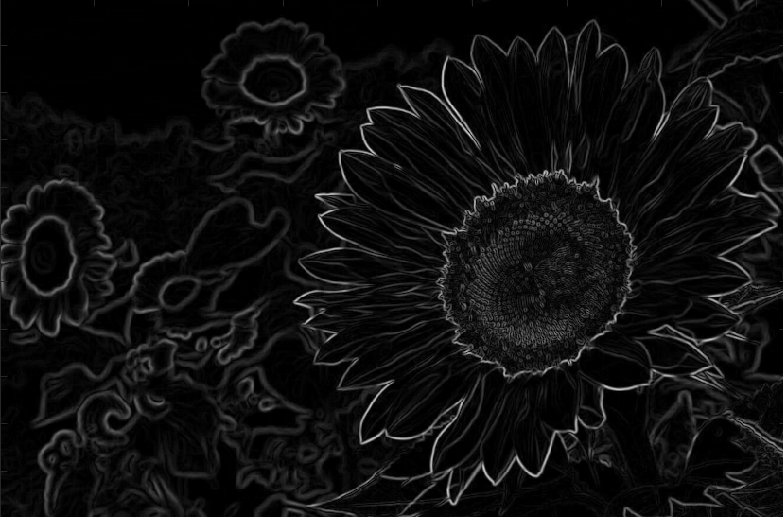
\includegraphics[width=\textwidth]{litreview/imageprocessing/linearfiltering/kernels/sunflowers_xy}
        \caption{Gradient Magnitude}
        \label{fig:hoz}
    \end{subfigure}
    \caption{Application of Sobel filters to find gradient magnitude of an image.}
    \label{fig:sobel_apply2}
  \end{figure}